\title{Proposal for the BSc. AI 2013 \\Final Thesis Project}
\author{
        O.R. Jozefzoon\\
                Department of Artificial Intelligence\\
       Student-- Faculty of Physics, Mathematics and Computer Science \\
        Amsterdam, North-Holland, \underline{The Netherlands}
}
\date{\today}

\documentclass[12pt ,twocolumn]{article}
\usepackage{wrapfig, graphicx, caption, sidecap}
\begin{document}
\maketitle
\bibliographystyle{acm} %Association for Computiny Machinery  bibliograhpic style

\section{Introduction}
The Amsterdam Museum has created a  Museum App for mobile phones,  which is an enhanced museum guidance system that uses trigger points, information nodes related to GEO points, to enrich the user with content during a tour around the city of Amsterdam. 

After experiencing the tour first hand we discussed our experience with a member of the museum experience developing staff. This led to the conclusion that an added feature was needed to improve the user experience of the tour. 

This is where the idea emerged of transforming the existing data from the tour in an augmented reality, a live, direct or indirect, view of a physical, real-world environment whose elements are augmented by computer-generated sensory input such as sound, video, graphics or GPS data also known as AR, experience, in which a user is able to find a given object, as described in the tour, by means of the method of highlighting recognized patterns, in realtime.

\paragraph{Outline}
The remainder of this article is organized as follows.
Section~\ref{literature review} gives account of previous work to determine what is already available as potential solutions. We then describe the missing aspects based on which we build our research question in section \ref{research question.}. In section \ref{method} we then outline the method used to answer the questions and present our added feature to an existing tour guidance application.  In section \ref{evaluation} we cover the evalution of our implementations and  finalize the proposal with a schedule in section \ref{plan}.

\section{Literature review}\label{literature review}
Many applicants of location-aware applications propose the use of trigger zones to activate content and the use of servers to perform object recognition. Even though, location-awareness by the use of trigger zones is a highly efficient manner to display or use content, this dependency does not allow much room flexibility of the application.
Lameira et al. (2011)~\cite{Lameira:2011:ROR:2037373.2037485} propose an application for real time object recognition without the use of a server. They reported that this method gives 
\begin{quotation}
“ fast feedback to the mobile user and, at the same time, has reasonable detection/identification rates. The fast feedback promotes a better interaction and co-operation between the user and the mobile application \end{quotation}
which, consequently, can be used to improve the quality of detection/identification.” 

Even though, we are not completely ignoring the value of a server, we also aim to limit the use of the server to a maximum and depend for the biggest part of our computations on the power of the mobile device. The reason for this decision is based on the fact that mobile device, nowadays, are improved, have increased computational power and are, thus, able to perform complex computations within a reasonable amount of time. This decision allows us to limit the use of a server to perform only the act of a storage facility for our required data and make our application as independent and as fast as possible. Independent in the sense that the application is not dependent of an internet-connection to connect with the server, once the data is stored, and as fast as possible in the sense that the computation does not depend on an external source, but is almost completely self-sufficient.

Amlacher et al. (2008)~\cite{Amlacher:2008:GOR:1409240.1409291} demonstrate in their paper a manner in which geo-indexed object recognition from experimental tracks and image in an urban scenario, extracts object hypotheses in the local context from both mobile image based appearance and GPS based positioning”. They reported 

\begin{quotation}
that geo-information provides a focus on the local object context that enables a meaningful selection of expected object hypotheses and therefore improves overall performance of urban object recognition.” 
\end{quotation}. These results are obtained with the use of the SIFT, a Scale-invariant feature transform algorithm used in computer vision to detect and describe local features in images. For our research we propose to use geo-indexed verification to check whether or not the assumptions, based on extracted object hypotheses conceptualized from text, made by our application are accurate. The result from the demonstration by Amlacher et al. (2008) provides us with a basis assumption to use geo-indexed data to improve the accuracy and coverage of our application. Furthermore, their research has shown that it is a well This means that we will incorporate SIFT as a object recognition algorithm to detect features in our visual content.

According to a research conducted by F\"{o}chler et al. (2005)~\cite{Fockler:2005:PMG:1149488.1149490} the use of a single-layer perceptron neuronal network is sufficient to achieve an object recognition accuracy of over 90\%. This accuracy rate is achieved with the use of a mobile phone. Following the findings of F\"{o}chler et al. we aim to reach the same accuracy on a mobile device. Even though, we are not yet certain if the use of a single-layer perceptron neural network is the most efficient manner to achieve the desired result in combination with our application such a high recognition rate is certainly desirable for the use of our application. We propose the use of an object recognition algorithm (SIFT), but without the use of an existing database of images. The application is supposed to recognize the object in real-time within a reasonable amount of time based on a conceptualized description of our textual data.

Furthermore, the use of a server creates a dependency from an external source, but with the improvement of mobile devices and object recognition algorithms this will not be necessary.
The client-side tracker as proposed by Gammeter et al. (2010)~\cite{eth_biwi_00782} in ‘Server-side object recognition and client-side object tracking for mobile augmented reality’ is a valuable device, which we will use to memorize the position of an object even when out of screen, using visual and sensor based cues. This client-side tracker is necessary because the user will be guided towards an object to be recognized. Gammeter et al. does not use GPS information for object recognition and tracking. We, on the other hand, will use GPS information for the verification of the results presented by the application and, combined with the compass on the mobile device, as a device to guide the user in to the desired direction. Our use of the GPS and Compass information will provide the application with a more robust base to guide the user and to co-operate with the object recognition algorithm.

The description of the architectural concepts needs some form of accepted base. For this task the Getty`s AAT\footnote{http://www.getty.edu/research/tools/vocabularies/aat/} can be used. 
AAT stands an acronym for Art and Architectural Thesaurus and is a
\begin{quotation}
controlled vocabulary used for describing items of art, architecture, and material culture. \\
... structured vocabulary of around 34,000 concepts, including 131,000 terms, descriptions, bibliographic citations, and other information relating to fine art, architecture, decorative arts, archival materials, and material 
culture.\footnote{Source: http://en.wikipedia.org/wiki/AAT}
\end{quotation}

\section{Research question.}\label{research question.}
Based on the presented literature and the established problem of the Amsterdam Museum we decided on the following research question:

What is a feasible method to transform contextualized textual architectural concepts into visual markers to be presented in real time as overlays in AR environments?

Our aim is to reduce the dependency of the triggers by implementing an application that provides a user with content based on an observation of an object in the real world (i.e. through a camera of the mobile phone) and on abstraction from a textual source (the concepts highlighted by the user in the Amsterdam Museum’s Tour). The transformation process from textual concept into the final marker will adapt AAT  descriptions of object/buildings, in combination with GEO data and compass information. In that way we  propose a new approach in which our content is activated by the input from the data (text/image) and afterwards verified using geo-location and compass data from the mobile device.  

\section{Method and approach}\label{method}
In order to achieve our goal, of creating a feasable model that transforms contextualized textual architectural concepts into visual markers to be presented in real time as overlays in AR environments, we will use the method of implementing and testing. 
In the first stage we will decide for a manner to  conceptualize the textual data to a model which will be useful for the transformation process. Here the conceptualization will be determined with the use of descriptions from the AAT and manually selected locations. The locations will serve as a reference- or pinpoints on which we will base our conceptualization. This conceptualization will be necesarry, because our algorithm has to be provided with a base to work on.
Once the correct representation of our data is determined we will start with the implementation of our application. The application will use the conceptualized data to present the user with the correct or clear description, as shown in figure ~\ref{fig:fig1}, of an object in the real world. In other words, the conceptualized textual data will be transformed into a usable model that can be used to recognize certain patterns in videoimages and highlights the recognized patterns in the screen of the user. 

When it seems as if the correct description is not provided, thus none or the wrong object are highlighted, we will explore the added feature of using the GPS and/or compass data for an extra verification. This verification might be necessary when the user, for example, does not find the object described or the application does not find a matching description for the object presented by the user. 

\begin{figure}

\includegraphics[scale=0.185]{AR_matching.png}
\captionsetup{font=scriptsize}
\caption{\\Image obtained from http://www.elipsead.com/mobile\_ar to demonstrate the eventual output, the highlighting of objects in an image.}
\label{fig:fig1}
\end{figure}
\section{Evaluation}\label{evaluation}
As mentioned beforehand, in this section we will describe how will the results of the research be evaluated? In a way this can be regarded as part of the method/approach, but it is important and therefore requires independent attention. 

The main evaluation will occur after finishing the implementation of the application. However, we will incorporate unit test in our code to make sure that we are not providing our application with incorrect data our malicious chunks of codes. The unit tests are necessary for our application, because malicious codes may corrupt the accuracy and might negatively affect the coverage.
	For our main evaluation real world testing will be necessary. This means that we will test if the application works as desired on the selected locations. If we are not provided with the desired results then we will have to decide whether the source of the error is our conceptualization of the text or whether the error could be found at the side of the object recognition algorithm(s) used. In case of the first we have to reconsider our conceptualization, in case of the latter an obvious reconsidering of algorithm will be necessary. We will probably mainly revise the algorithms, because the conceptualization will be given a fair amount of (re-) consideration and once the decision is made for an acceptable representation it is our task to implement a suiting algorithm.

\section{Plan}\label{plan}

In this section we will explicate the order in which the activities following from the above will be carried out in time. As well as how much time (effort in terms of hours or days) will be allocated to each task. \\\\ Figure 2 describes the plan we have concluded for the proceedings of this paper. At this points we do not expect any hurdles on our path, because the implementations will be straight forward. It will however be possible that their occur some delay understanding the SIFT and the AAT, but these delays are already take under consideration at the creation of this plan.
\begin{figure}

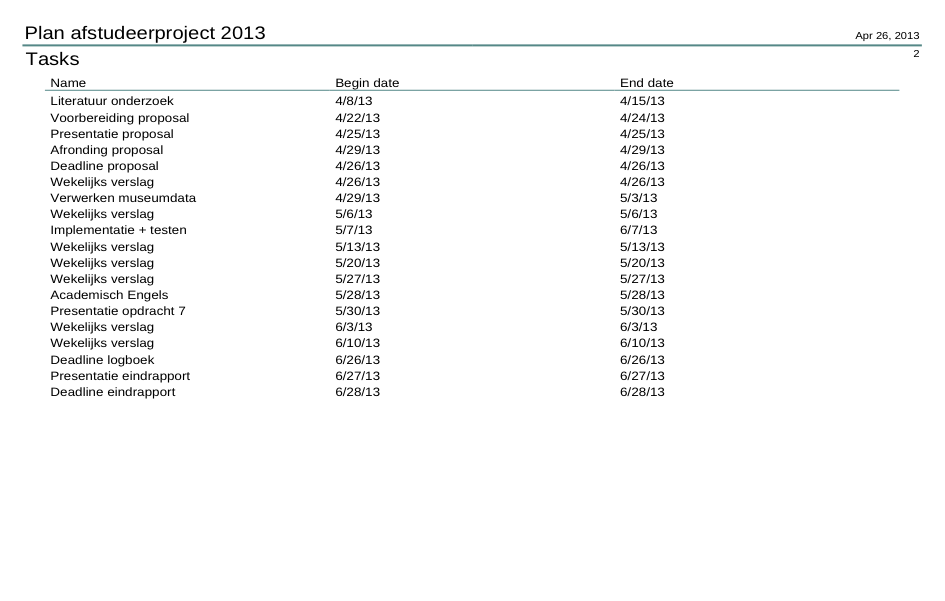
\includegraphics[scale=0.80]{plan.png}

\captionsetup{font=scriptsize}
\caption{Planning BSc scriptie 2013 - Jozefzoon} 
\end{figure}
\newpage
\bibliography{main}
\end{document}
O.R. Jozefzoon 2013